% Chapter 4

\chapter{Neural network design and implementation} % Main chapter title

\label{Chapter4} % For referencing the chapter elsewhere, use \ref{Chapter4} 

%----------------------------------------------------------------------------------------
\section{External libraries}
DeepMiRNA has been developed using \emph{Python3}. The \emph{requirements.txt} file, present in the project root directory, contains names and versions of all libraries used for the implementation. In particular, we used \emph{Pandas} and \emph{Numpy} for the preprocessing step and the datasets preparation together with \emph{RNA} (the Python version of the Vienna Cofold) and \emph{Biopython} to parse .fasta files and convert them to .csv. 

Implementation of the neural network was done with \emph{Keras}\cite{keras} using \emph{Tensorflow} backend\cite{tensorflow}. Keras is an open-source neural-network library capable of running on top of TensorFlow, Theano and other major deep learning frameworks. Keras contains numerous implementations of commonly used NN building blocks such as layers, optimizers or activation functions and it aims at being user-friendly, modular and extensible. However, Keras, which is now fully supported in the Tensorflow's core library, has been conceived more as an interface than a standalone framework. 

We opted for the use of this library because it offers a higher-level, more intuitive set of abstractions that makes it easier to develop deep learning models.    

\section{Choosing the right model}
Building deep learning applications in the real world is a never-ending process of selecting and refining the right elements of a specific solution. Among those elements, the selection of the correct model and the right structure of the training dataset are, arguably, the two most important decisions that any data scientist needs to make when designing deep learning solutions. How to decide what deep learning model to use for a specific problem? How do we know whether we are using the correct training dataset or we should gather more data? Those questions are the common denominator across all stages of the life cycle of a deep learning application. Even though there is no magic answer to those questions, there are several ideas that could guide the decision process. 

First of all we need to start identifying the correct baseline model, in particular we should select what type of networks suits more the input dataset. In the case of miRNA targets predictions the topological structure of the available data are strictly correlated to the vectorization method selected. If we opt for the one-hot encoding that maps duplexes into fixed-size vectors, we should be thinking of using a feed-forward network with inter layer connectivity. While, if we select the Dna2Vec approach that transforms each duplex into a matrix, then the problem could be tackled using convolutional neural networks (CNN)\cite{dl}.  

The second part concerns the selection of the optimization algorithm to use. The most popular are, arguably, SGD (Stochastic Gradient Descent) and its variation using momentum or learning decay, and Adam. The latter, in particular, is very often used combined with CNNs.

As mentioned in chapter \ref{Chapter3} DeepMiRNA uses 2 different neural network for the training stage according to the chosen data representation: a regular feed-forward network for the one-hot encoded sequences and a CNN for the Dna2Vec encoded duplexes. 

\subsection{The feed-forward network} 
The feed-forward network is a very simple neural network consisting in 5 dense hidden layers, comprising rectifier activation function ReLU nodes, each followed by a dropout layer. Dropout\cite{dropout} is a regularization technique used to prevent overfitting. In this thesis, the dropout rate has been set to $0.8$ meaning that $20\%$ of the neurons in each layer are ignored (i.e set to 0). Basically this implies that their contribution to the activation of downstream (i.e. next layer) neurons  is temporally removed on the forward pass and weight update is not applied on the backward pass.   

The reason why this process can be useful is that, while a neural network learns, neuron weights settle into their context within the network. Those weights are tuned for specific features providing some specialization. Neighboring neurons become to rely on this specialization, which, if taken too far, can result in a fragile model too specialized on the training data.Hence, if neurons are randomly dropped out of the network during training, other neurons will have to step in and handle the representation required to make predictions for the missing neurons. This is believed to result in multiple independent internal representations being learned by the network.
The effect is that the network becomes less sensitive to the specific weights of neurons and results in a model capable of better generalization and less likely to overfit the training data.    

The output layer is composed of one sigmoid node that returns a value between 0 and 1 corresponding to the final score prediction. The resulting architecture can be visualized in figure \ref{fig:NN}.

\begin{figure}[hbt!]
	\centering
	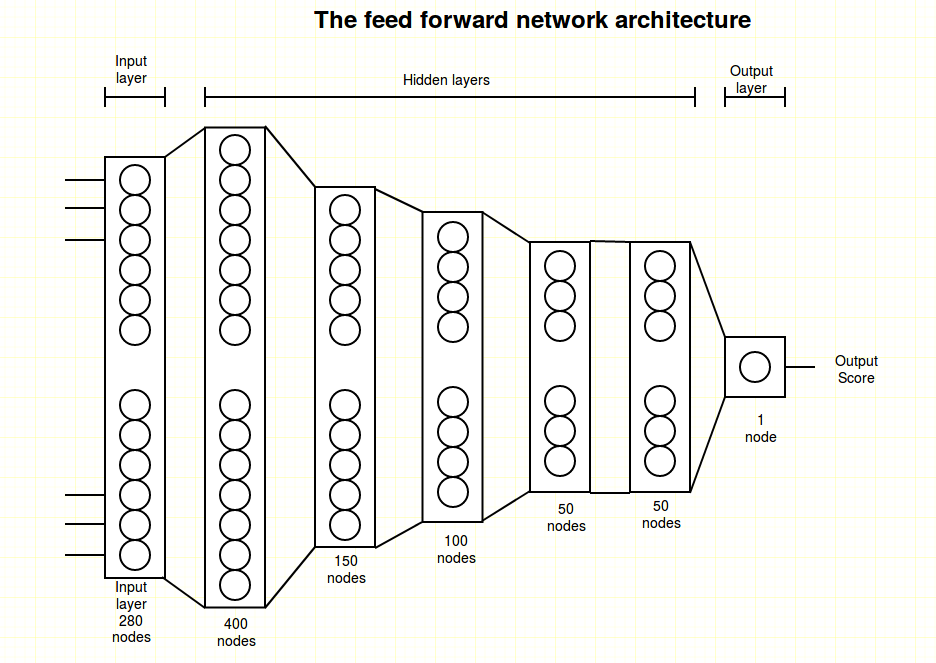
\includegraphics[width=\textwidth, height=0.52\textheight]{Figures/NN}
	\caption{\textbf{The Neural Netkork}. The first hidden layer increases the dimensionality of the input allowing the representation of data in a more complex feature space. There is debate in the machine learning community regarding the need of such over-completion layers, as they do not necessarily improve the accuracy whilst making the learning process slower. Considering that the relatively low number of inputs of the proposed network allows a fast training procedure, we opted to include this higher dimension layer to give the network the chance of identifying more complex patterns.}
	\label{fig:NN}
\end{figure}
 

As optimization function we chose the Adam optimizer with the following parameters:

\begin{itemize}
	\item learning rate = 0.002;
	\item beta\_1 = 0.9;
	\item beta\_2 = 0.999;
	\item epsilon = $1e-8$;
	\item decay = 0
\end{itemize}